%----------------------------------------------------------------------------------------
%	PACKAGES & THEMES
%----------------------------------------------------------------------------------------

\pdfminorversion=4
\documentclass[8pt]{beamer}

\usepackage{etex}
\mode<presentation> {

\usetheme{Vilanova}

}



\usepackage[french]{babel}
\usepackage[utf8]{inputenc}
\usepackage{array}
\usepackage{chronology}
\let\CHRONOLOGY\chronology
\let\endCHRONOLOGY\endchronology
\def\chronology{\shorthandoff{;}\CHRONOLOGY}
\def\endchronology{\endCHRONOLOGY\shorthandon{;}}
\usepackage{pstricks}
\usepackage{graphicx}
\usepackage{booktabs}
\usepackage{amsmath,amssymb,amsthm}
\usepackage{xcolor}
\usepackage{tikz}
\usetikzlibrary{arrows}
\usepackage{pifont}

\usepackage{listings,color}

\definecolor{listcomment}{rgb}{0.0,0.5,0.0}
\definecolor{listkeyword}{rgb}{0.0,0.0,0.5}
\definecolor{listnumbers}{gray}{0.65}
\definecolor{listlightgray}{gray}{0.955}
\definecolor{listwhite}{gray}{1.0}


\AtBeginSection[]
{
\addtocounter{framenumber}{-1}
\begin{frame}
\frametitle{Sommaire}
\tableofcontents[currentsection]
\end{frame}}

\title{Orfeo ToolBox}
\subtitle{Un logiciel libre pour le traitement d'images de télédétection.}
\author{Victor Poughon \texttt{\textless victor.poughon@cnes.fr\textgreater}}
\date{Mercredi 29 juin 2016}

\pgfdeclareimage[height=96mm,width=130mm]{background}{art/fondsClairSansLogo}
\pgfdeclareimage[height=0.2cm]{cc}{art/CC-licence.png}
\setbeamertemplate{background}{\pgfuseimage{background}}
\pgfdeclareimage[height=0.6cm]{logoIncrust}{art/logoIncrust}
\pgfdeclareimage[height=0.6cm]{logo_cnes}{art/logo_cnes}
\logo{
\begin{tabular}{p{0.22\textwidth}p{0.58\textwidth}p{0.1\textwidth}p{0.1\textwidth}}
\href{http://www.cnes.fr}{\pgfuseimage{logo_cnes}}
& \vspace{-0.03\textwidth} \scriptsize{} % date and event here
& \href{http://creativecommons.org/licenses/by-sa/3.0/}{\pgfuseimage{cc}} & \href{http://www.orfeo-toolbox.org}{\pgfuseimage{logoIncrust}}\\
\end{tabular}
}

\titlegraphic{\vspace*{-5em}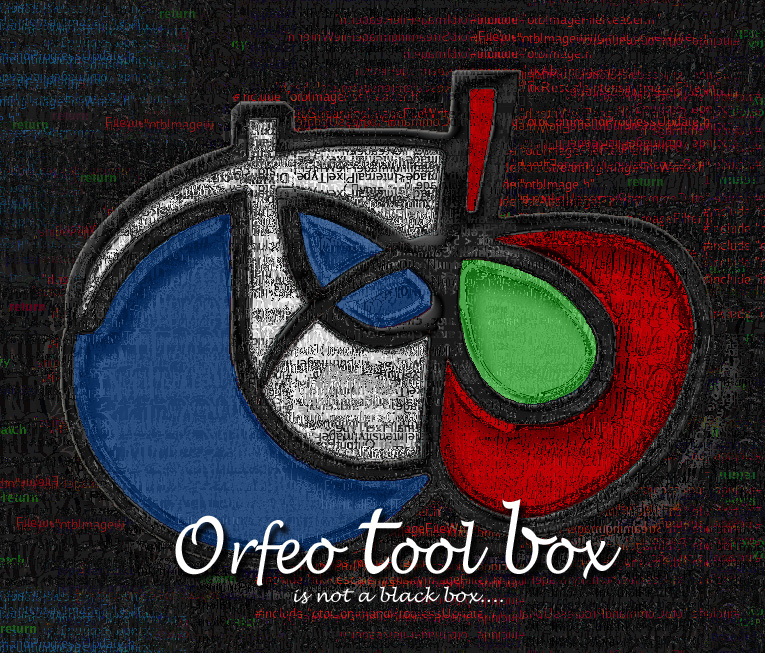
\includegraphics[width=.4\textwidth]{art/LOGOTB_blackbox.png}}

\begin{document}
\begin{frame}
\titlepage
\end{frame}

\section{Introduction}

\begin{frame}
\frametitle{Si vous ne retenez qu'une planche\ldots}
\begin{block}{L'Orfeo ToolBox est:}
\begin{itemize}
\item Une \textbf{bibliothèque de traitement d'images} pour la télédétection
\item \textbf{Un logiciel libre} diffusé sous licence CeCILL-v2 (équivalent à la GPL)
\item \textbf{Financée et développée par le CNES} (principalement)
\item Écrite en \textbf{C++} sur la base d'\href{www.itk.org}{ITK} (imagerie médicale)
\item Construite sur les épaules de géants (ITK, GDAL, OSSIM, OpenCV\ldots)
\item Conçue pour traiter de \textbf{gros volumes de données} de manière transparente grâce au traitement par morceaux et à la parallélisation
\end{itemize}
\end{block}

\begin{center}
{\huge\textcolor{red}{\href{http://www.orfeo-toolbox.org}{orfeo-toolbox.org}}}
\end{center}

\end{frame}

\begin{frame}
\frametitle{Pourquoi un logiciel libre ?}

\begin{block}{Diffusion maximale}
L'OTB est un logiciel à destination de tous les utilisateurs d'imagerie
spatiale. Sa diffusion large contribue au rayonnement des missions (Pléiades, Sentinels\ldots)
\end{block}

\begin{block}{Qualité et efficacité}
Le domaine fonctionnel de l'OTB est vaste, son développement nécessite du temps
et de l'expertise. L'ouverture des sources favorise:
\begin{itemize}
\item L'appropriation et la validation par la communauté des utilisateurs,
\item Les contributions et les corrections de bugs par les utilisateurs,
\item La dissémination sur de multiples plateformes.
\end{itemize}
\end{block}

\begin{block}{Démarche scientifique}
L'OTB capitalise une partie de la R\&D du CNES en extraction d'information, l'ouverture des sources permet une démarche de \textbf{recherche reproductible}.
\end{block}

\end{frame}

\section{Fonctionnalités}

\begin{frame}
\frametitle{Les grandes familles de fonctionnalités dans l'OTB (forcément incomplètes)}

\begin{block}{Pré-traitements}
\begin{itemize}
\item Calibration radiométrique, ortho-rectification, reprojection (raster et vecteur), pan-sharpening, stéréo-rectification,
\item Capteurs supportés: Sentinels, Pléiades, SPOT6, SPOT5, capteurs DigitalGlobe
\item Modélisation géométrique fournie par OSSIM, support de MNT SRTM ou GeoTIFF
\end{itemize}
\end{block}

\begin{block}{Manipulation d'images et de vecteurs}
\begin{itemize}
\item Formats supportés par Gdal (raster et vecteur), conversion raster/vecteur
\item Extraction de ROI, de bandes spectrales, concaténation ou séparation des bandes spectrales,
\item calcul mathématiques entre bandes, color mapping, optimisation du contraste
\item Filtrage linéaire, morphologie mathématique,
\end{itemize}
\end{block}
\end{frame}

\begin{frame}
\frametitle{Les grandes familles de fonctionnalités dans l'OTB (forcément incomplète)}

\begin{block}{Détection d'éléments saillants et calcul de primitives}
\begin{itemize}
\item Détection de contours, points d'intérêt SIFT et SURF, lignes, angles droits
\item Indices radiométriques, indices de textures (Haralick, SFS, PanTex)
\item Descripteurs statistiques locaux (moments de Flusser, HOG)
\item Matching de points d'intérêts
\end{itemize}
\end{block}

\begin{block}{Détection de changement}
\begin{itemize}
\item Algorithme classique avec métrique de comparaison d'images,
\item Algorithme MAD (Multivariate Alteration Detector)
\end{itemize}
\end{block}

\begin{block}{Réduction de la dimension, traitement hyperspectraux}
\begin{itemize}
\item Réduction de la dimension: PCA, NAPCA, ICA, MAF \ldots
\item Estimation de la dimension et extraction des pixels purs: algorithme VCA
\end{itemize}
\end{block}

\end{frame}

\begin{frame}
\frametitle{Les grandes familles de fonctionnalités dans l'OTB (forcément incomplète)}
\begin{block}{Segmentation}
\begin{itemize}
\item Algorithmes de segmentation Connected Components, MeanShift, Ligne de partage des eaux
\item Méthodologie pour une application large échelle,
\item Représentation vectorielles et raster des résultats, avec capacités d'analyse objet
\end{itemize}
\end{block}

\begin{block}{Classification}
\begin{itemize}
\item Supervision et classification d'images avec 9 algorithmes au choix (dont SVM et forêts aléatoires)
\item Fusion et régularisation de cartes de classification
\item Clustering de type K-Means ou carte de Kogonen
\item Classification objets (segments issus d'une segmentation)
\end{itemize}
\end{block}
\end{frame}

\begin{frame}
\frametitle{Flexibilité, passage à l'échelle: \textit{Pipeline}, \textit{Streaming} et \textit{multithreading}}

\begin{block}{Le modèle de \textit{Pipeline}}
\begin{center}
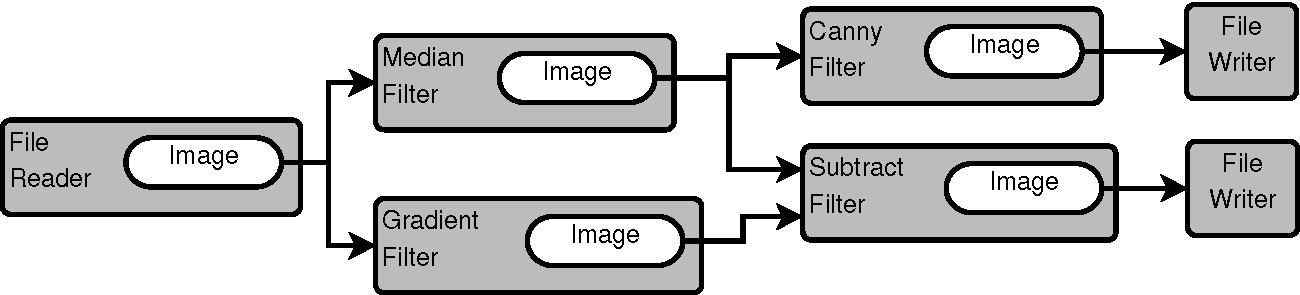
\includegraphics[width=0.7\textwidth]{art/ProcessObjectDataObject.png}
\end{center}
\end{block}
\vspace{-0.5cm}
\begin{block}{\textit{Streaming}}
\begin{center}
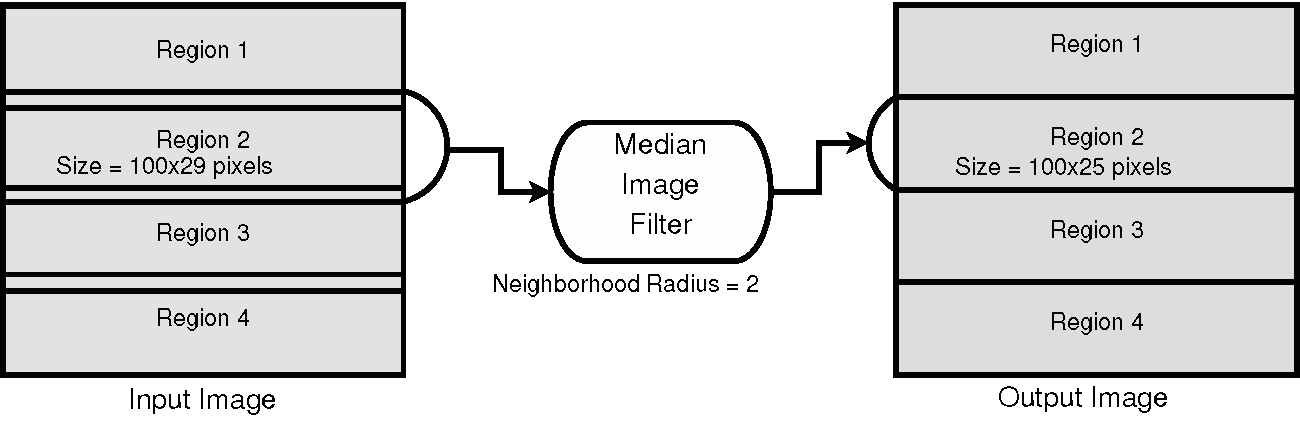
\includegraphics[width=0.7\textwidth]{art/StreamingImageDiagram.png}
\end{center}
\end{block}
\vspace{-0.5cm}
\begin{center}
\tiny{source: http://www.aosabook.org/en/itk.html}
\end{center}
\end{frame}

\begin{frame}
\frametitle{Proche de l'état de l'art}
\begin{itemize}
\item Veille technologique de l'équipe de développement
\item Implémentations d'algorithmes récents d'après publication. Ex.: profils morphologiques, segmentation MeanShift, textures de Haralick, points d'intérêt SURF \ldots
\item Implémentations de références contribuées par les auteurs de certains travaux en support à leur publication. Ex.: Large Scale MeanShift, fusion bayésienne, détection d'objets \ldots
\item Veille pour bénéficier des avancées des logiciels tiers. Ex.: algorithmes de \textit{machine learning} d'OpenCV,
\item Souvent: pour une même brique fonctionnelle, plusieurs algorithmes de complexités différentes disponibles sous une même interface.
\end{itemize}
\end{frame}

\begin{frame}[plain]
\hspace*{-11mm}
    \includegraphics[keepaspectratio,height=1.1\paperheight]{art/mayotte2012.png}
\end{frame}

\vspace*{-6.5mm}
\begin{frame}[plain]
\hspace*{-11mm}
    \includegraphics[keepaspectratio,height=1.1\paperheight]{art/mayotte2013.png}
\end{frame}

\vspace*{-6.5mm}
\begin{frame}[plain]
\hspace*{-11mm}
    \includegraphics[keepaspectratio,height=1.1\paperheight]{art/mayotte_mad.png}
\end{frame}

\vspace*{-6.5mm}
\begin{frame}[plain]
\hspace*{-11mm}
\includegraphics[keepaspectratio,height=1.1\paperheight]{art/saint_paul_lsd.png}
\end{frame}

\vspace*{-6.5mm}
\begin{frame}[plain]
\hspace*{-11mm}
    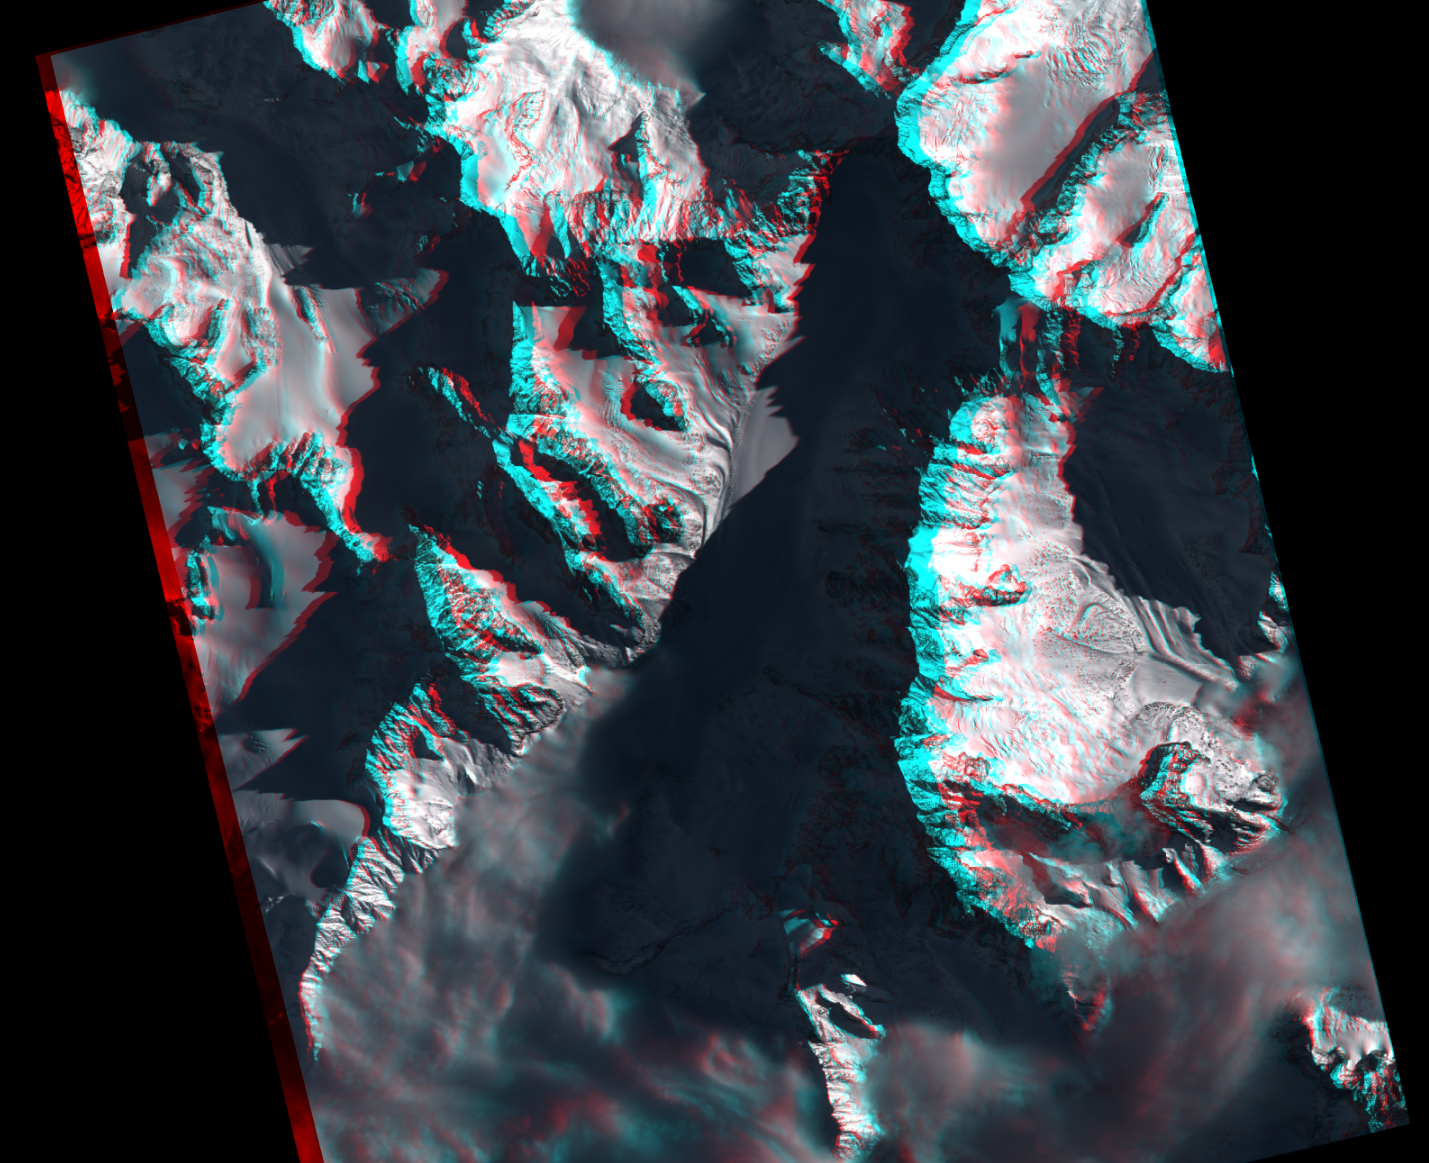
\includegraphics[keepaspectratio,width=1.005\paperwidth,height=1.1\paperheight]{art/argentiere_anaglyphe.png}
\end{frame}

\begin{frame}
\frametitle{Comment utiliser l'Orfeo ToolBox?}
\vspace{-0.5cm}
\begin{center}
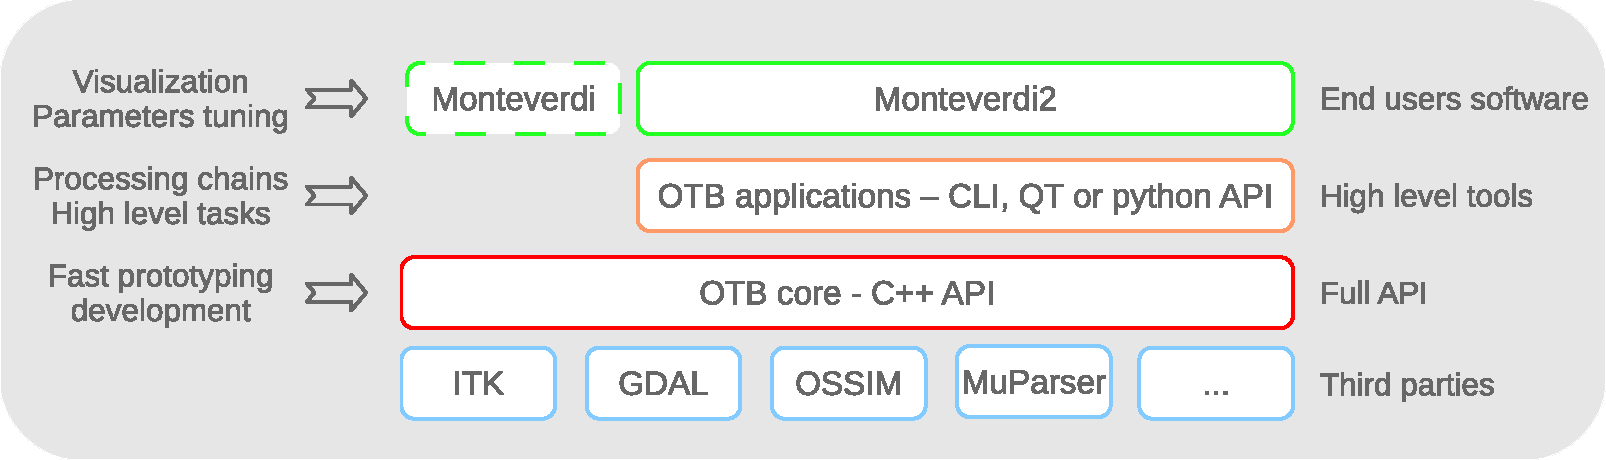
\includegraphics[width=\textwidth]{art/sandwich.pdf}
\end{center}
\vspace{-0.5cm}
\begin{block}{Écrire son propre code}
 Flexible, à partir de la bibliothèque OTB, demande une connaissance en C++
\end{block}
\begin{block}{Utiliser les applications OTB}
 Fonctions de haut niveau (par ex. segmentation), appelable en ligne de commande, via une interface graphique, ou depuis Python. Peut être étendue (création d'applications)
\end{block}
\begin{block}{Utiliser le module Monteverdi (IHM)}
Visualisation, gestion persistante des données, \textcolor{red}{Accès à l'ensemble des applications}
\end{block}
\end{frame}

\begin{frame}[fragile]
\frametitle{Show me the code!}
\begin{lstlisting}[language=c++,breaklines=true,breakatwhitespace=true,frame = tb,framerule = 0.25pt,fontadjust,backgroundcolor={\color{listlightgray}},basicstyle = {\ttfamily\tiny},keywordstyle = {\ttfamily\color{listkeyword}\textbf},identifierstyle = {\ttfamily},commentstyle = {\ttfamily\color{listcomment}\textit},stringstyle = {\ttfamily},showstringspaces = false,showtabs = false,numbers = none,numbersep = 2pt, numberstyle={\ttfamily\color{listnumbers}},tabsize = 2]
#include "otbImage.h"
#include "otbImageFileReader.h"
#include "otbImageFileWriter.h"
#include "itkCannyEdgeDetectionImageFilter.h"
#include "itkRescaleIntensityImageFilter.h"

int main(int argc, char * argv[])
{
  typedef double                      PixelType;
  typedef otb::Image<PixelType>       ImageType;
  
  typedef unsigned char               OutputPixelType;
  typedef otb::Image<OutputPixelType> OutputImageType;

  typedef otb::ImageFileReader<ImageType> ReaderType;
  ReaderType::Pointer reader = ReaderType::New();

  reader->SetFileName(argv[1]);

  typedef itk::CannyEdgeDetectionImageFilter
  <ImageType, ImageType> FilterType;
  FilterType::Pointer filter = FilterType::New();

  filter->SetInput(reader->GetOutput());

  typedef otb::ImageFileWriter<OutputImageType> WriterType;
  WriterType::Pointer writer = WriterType::New();

  writer->SetFileName(argv[2]);
  
  writer->SetInput(filter->GetOutput());

  writer->Update();
}
\end{lstlisting}
\end{frame}

\begin{frame}
\frametitle{Les applications: codées une fois, utilisables partout}
\begin{columns}
\column{0.5\textwidth}
\begin{itemize}
\item 87 applications sont livrées avec l'OTB
\item 1 application $=$ 1 librairie dynamique (plugin)
\item Les applications sont auto-descriptives et auto-documentées
\item Les applications peuvent etre étendues en dehors de l'OTB
\item Plusieurs interfaces sont disponibles pour utiliser les plugins:
\begin{itemize}
  \item Ligne de commande
  \item Interface Qt auto-générée
  \item Python
\end{itemize}
\item Les applications sont conçues pour une intégration facilitée dans des systèmes externes
\end{itemize}
\column{0.5\textwidth}
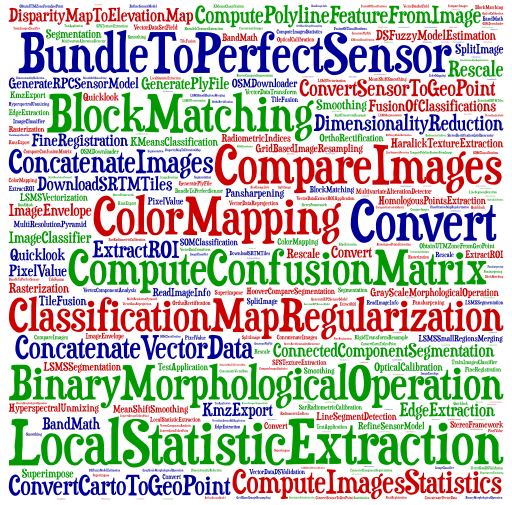
\includegraphics[width=\textwidth]{art/cloud_applications.png}
\end{columns}
\end{frame}



\begin{frame}[fragile]
\frametitle{Applications: appel depuis la ligne de commande}
\begin{scriptsize}
\vspace{-0.5cm}\begin{verbatim}
$ otbcli_OrthoRectification 

ERROR: Waiting for at least one parameter...
This is the OrthoRectification application, version 5.2.1
This application allows to ortho-rectify optical images from supported sensors.

Complete documentation: http://www.orfeo-toolbox.org/Applications/OrthoRectification.html

Parameters: 
        -progress                <boolean>        Report progress 
MISSING -io.in                   <string>         Input Image  (mandatory)
MISSING -io.out                  <string> [pixel] Output Image  [pixel=uint8/uint16/int16/uint32/int32/float/double] (default value is float) (mandatory)
        -map                     <string>         Output Cartographic Map Projection [utm/lambert2/lambert93/wgs/epsg] (mandatory, default value is utm)
        -map.utm.zone            <int32>          Zone number  (mandatory, default value is 31)
        -map.utm.northhem        <boolean>        Northern Hemisphere  (optional, off by default)
        -map.epsg.code           <int32>          EPSG Code  (mandatory, default value is 4326)
        -outputs.mode            <string>         Parameters estimation modes [auto/autosize/autospacing/outputroi/orthofit] (mandatory, default value is auto)
MISSING -outputs.ulx             <float>          Upper Left X  (mandatory)
MISSING -outputs.uly             <float>          Upper Left Y  (mandatory)
MISSING -outputs.sizex           <int32>          Size X  (mandatory)
MISSING -outputs.sizey           <int32>          Size Y  (mandatory)
MISSING -outputs.spacingx        <float>          Pixel Size X  (mandatory)
MISSING -outputs.spacingy        <float>          Pixel Size Y  (mandatory)
        -outputs.lrx             <float>          Lower right X  (optional, off by default)
        -outputs.lry             <float>          Lower right Y  (optional, off by default)
        -outputs.ortho           <string>         Model ortho-image  (optional, off by default)
        -outputs.isotropic       <boolean>        Force isotropic spacing by default  (optional, on by default)
        -outputs.default         <float>          Default pixel value  (optional, on by default, default value is 0)
        -elev.dem                <string>         DEM directory  (optional, off by default)
        -elev.geoid              <string>         Geoid File  (optional, off by default)
        -elev.default            <float>          Default elevation  (mandatory, default value is 0)
        -interpolator            <string>         Interpolation [bco/nn/linear] (mandatory, default value is bco)
\end{verbatim}
\end{scriptsize}
\end{frame}

\begin{frame}[fragile]
\frametitle{Applications: appel depuis l'interface Qt auto-générée (paramètres)}
\begin{center}
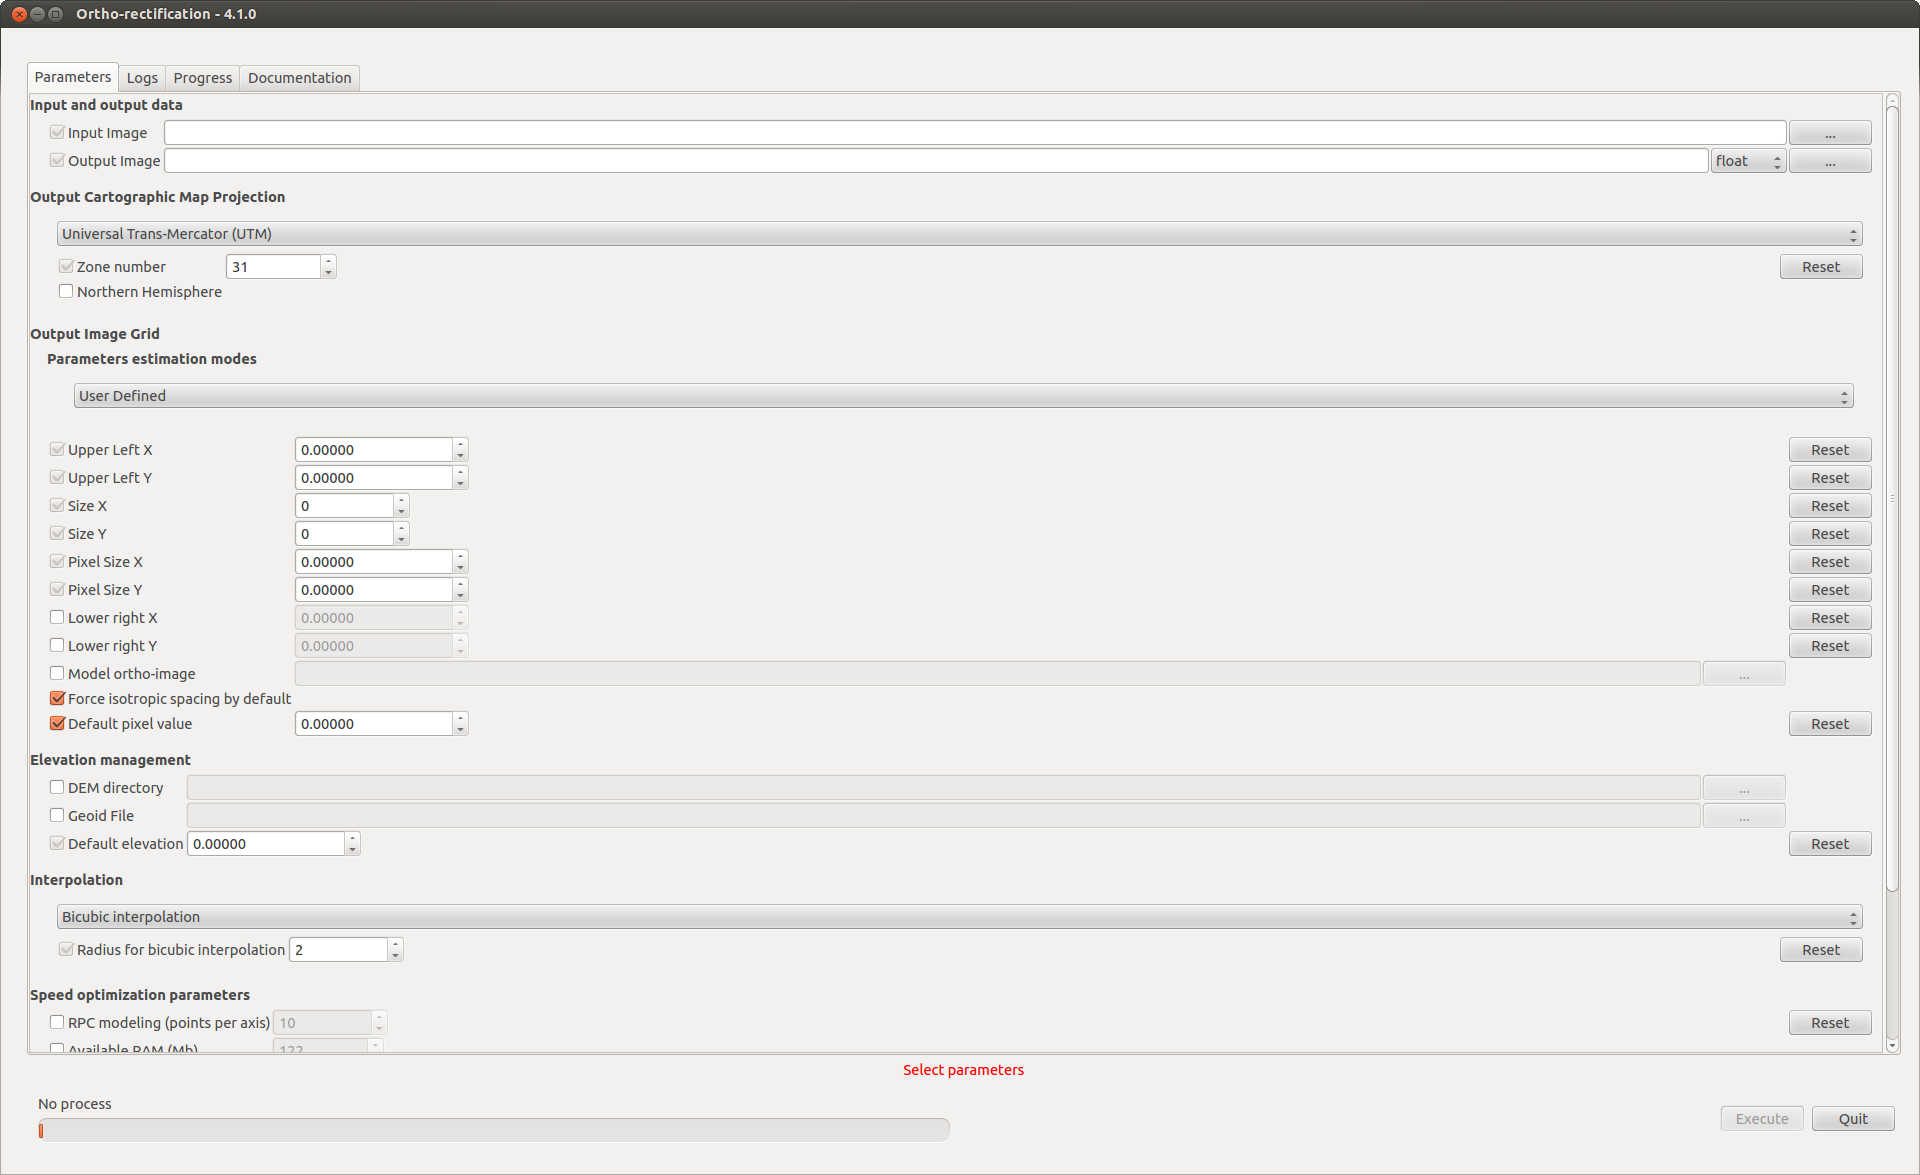
\includegraphics[width=0.9\textwidth]{art/app_parameters.png}
\end{center}
\end{frame}


\begin{frame}[fragile]
\frametitle{Applications: appel depuis l'interface Qt auto-générée (documentation)}
\begin{center}
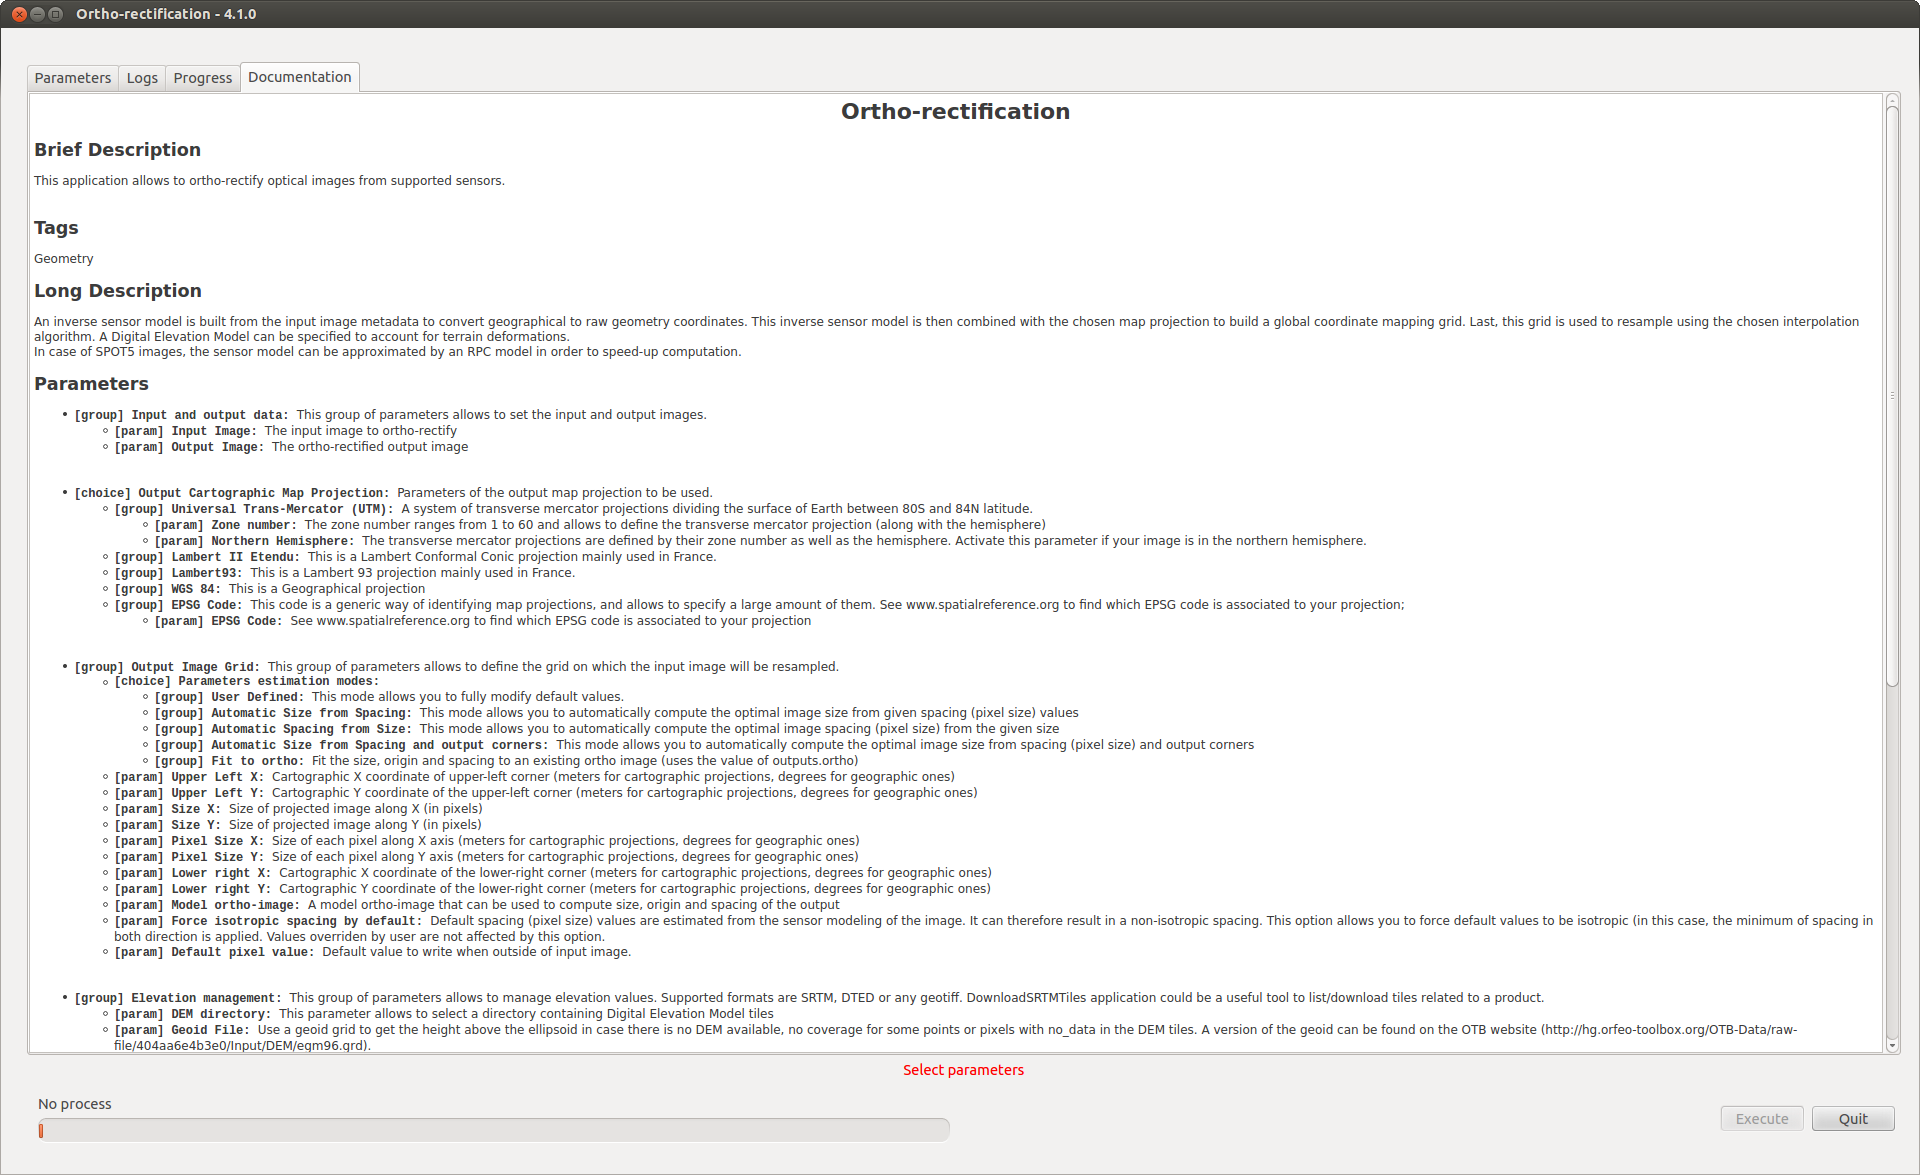
\includegraphics[width=0.9\textwidth]{art/app_doc.png}
\end{center}
\end{frame}

\begin{frame}[fragile]
\frametitle{Applications: appel depuis l'interface Python}
\begin{lstlisting}[language=python,breaklines=true,breakatwhitespace=true,frame = tb,framerule = 0.25pt,fontadjust,backgroundcolor={\color{listlightgray}},basicstyle = {\ttfamily\tiny},keywordstyle = {\ttfamily\color{listkeyword}\textbf},identifierstyle = {\ttfamily},commentstyle = {\ttfamily\color{listcomment}\textit},stringstyle = {\ttfamily},showstringspaces = false,showtabs = false,numbers = none,numbersep = 6pt, numberstyle={\ttfamily\color{listnumbers}},tabsize = 2]
#!/usr/bin/python 
 
# Import the otb applications package 
import otbApplication 
 
# The following line creates an instance of the OrthoRectification application 
OrthoRectification = otb.Registry.CreateApplication("OrthoRectification") 
 
# The following lines set all the application parameters: 
OrthoRectification.IO.IN = "QB_TOULOUSE_MUL_Extract_500_500.tif"
OrthoRectification.IO.OUT = "QB_Toulouse_ortho.tif"
 
app.MAP = 'epsg'
app.MAP.EPSG.CODE = 32768

# The following line execute the application 
OrthoRectification.ExecuteAndWriteOutput()
\end{lstlisting}
\end{frame}


\begin{frame}
\frametitle{Monteverdi (accès aux applications OTB)}
\begin{minipage}[t][6cm][t]{\textwidth}
\begin{center}
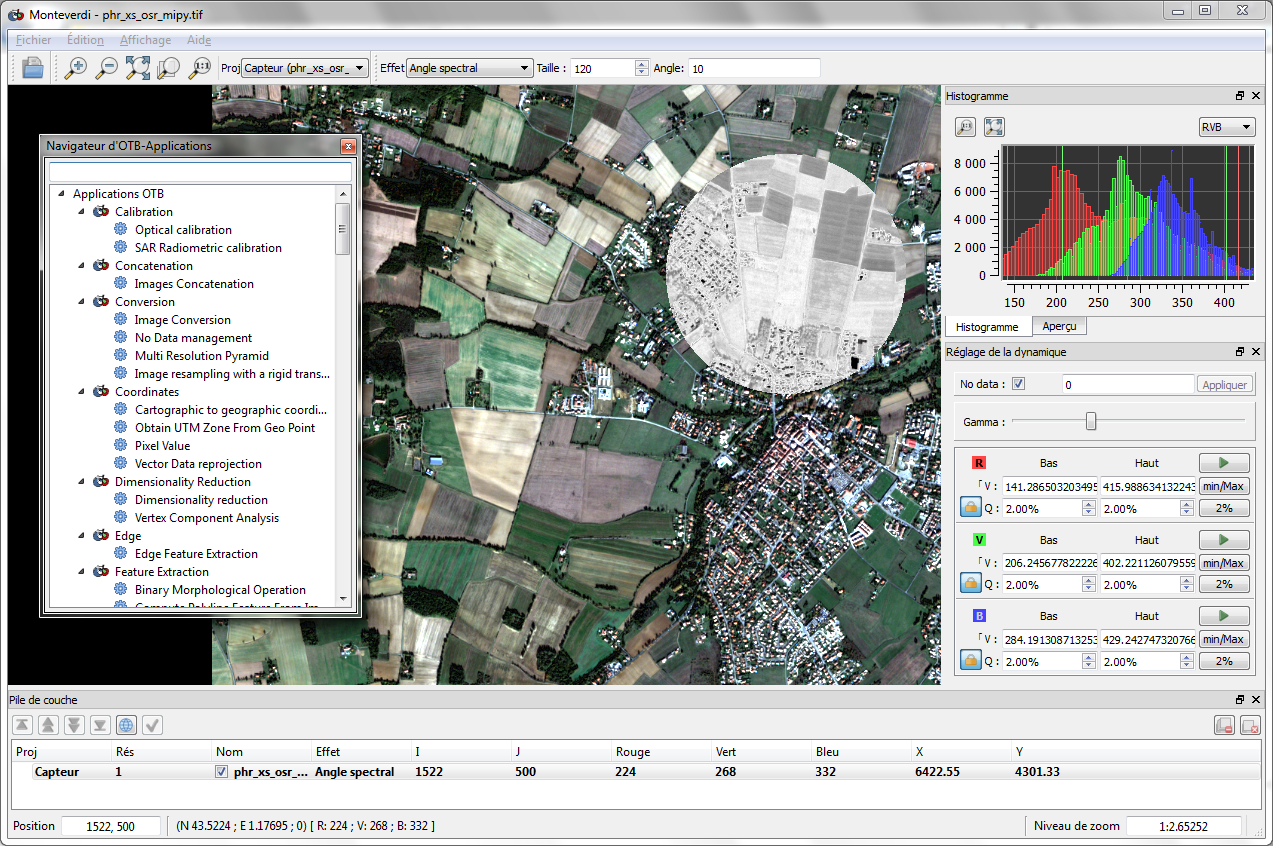
\includegraphics[width=1.0\textwidth]{art/monteverdi.png}
\end{center}
\end{minipage}
\end{frame}

%\vspace*{-3.0mm}
\begin{frame}
  \frametitle{QGIS (accès aux applications OTB)}
\begin{minipage}[t][6cm][t]{\textwidth}
\begin{center}
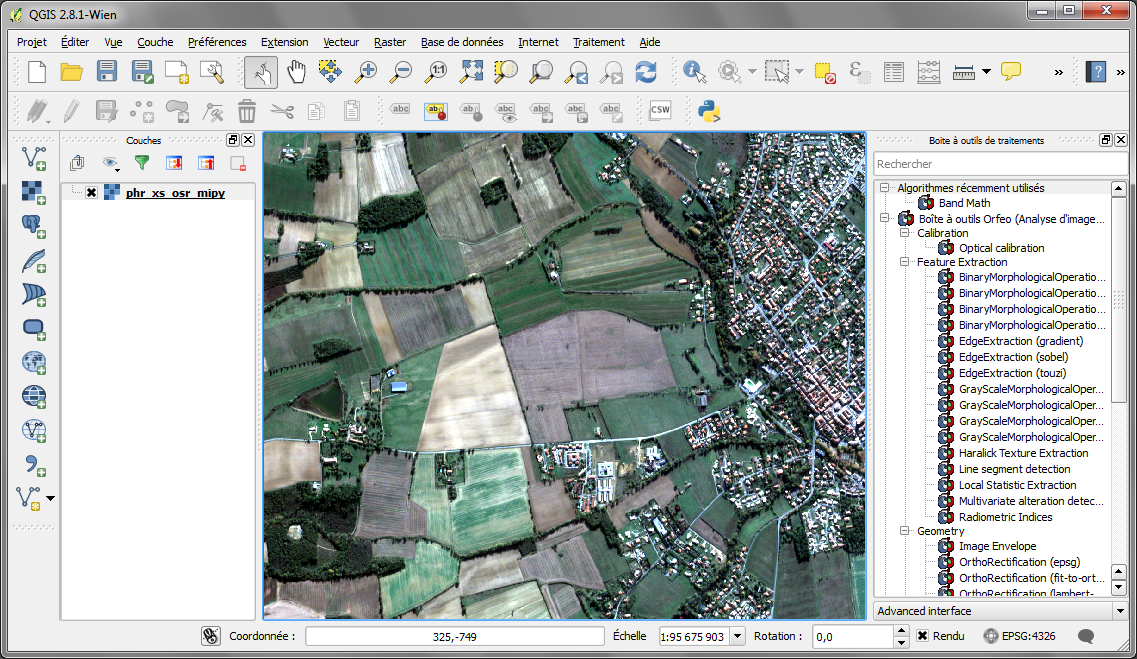
\includegraphics[width=1\textwidth]{art/otb_in_qgis.png}
\end{center}
\end{minipage}
\end{frame}

\section{Quoi de neuf depuis 5.0 ?}

\begin{frame}
\frametitle{5.0 (Mai 2015)}
\begin{block}{Modularité}
\begin{itemize}
\item Une meilleure organisation du code, en modules cohérents (124 modules et
    16 groupes) contenants sources, tests et applications.
\item Gestion des dépendances
\item Contributions externes: \url{https://www.orfeo-toolbox.org/external-projects/}
\end{itemize}
\end{block}

\begin{block}{SuperBuild}
\begin{itemize}
\item Il n'y a plus de logiciels tiers dans l'OTB
\item Le Superbuild, télécharge, configure, compile et installe les dépendances
\item Il existe également un mode \textit{offline} pour compiler l'OTB sans
  accès internet (en avion par exemple).
\end{itemize}
\end{block}
\end{frame}

\begin{frame}
\frametitle{Gouvernance ouverte: Project Steering Committee}
\begin{block}{Genèse du PSC}
  \begin{itemize}
  \item Jusqu'en 2015: l'OTB, un logiciel à sources ouvertes
  \item En mars 2015: l'OTB devient un logiciel libre, le CNES nomme un PSC initial
  \end{itemize}
\end{block}
\begin{block}{Un club de développeurs, pas de décideurs}
  \begin{itemize}
  \item Pilotage haut niveau du projet, roadmaps, communication, planification
  \item Vote les RFCs: Tous les membres ont le même poids dans les votes ($\pm 1$, $\pm 0$)
  \item Les sièges n'expirent pas, sortie par démission ou vote d'expulsion
  \item Le PSC n'est pas une entité légale et n'a pas de moyens propres
  \end{itemize}
\end{block}
\begin{block}{En chiffres}
  \begin{itemize}
  \item 5 membres de 4 entités différentes
  \item 2 release sous l'égide du PSC (5.2, 5.4)
  \item 3 meetings en ligne (logs publics)
  \end{itemize}
\end{block}
\end{frame}

\begin{frame}
\frametitle{5.2 (Décembre 2015)}
\begin{block}{OTB}
\begin{itemize}
\item Nouvelles applications pour le traitement SAR (polarimétrie, radiométrie, speckle)
\item Support des produits Sentinel-1
\item Amélioration accès OTB en Python
\item Compatibilité avec GDAL 2.0 et support des images Sentinel-2
\item \ldots
\end{itemize}
\end{block}

\begin{block}{Monteverdi 3.0}
\begin{itemize}
\item Affichage mosaïque d'images ou série multi-temporelle
\item Outils de visualisation performants (contraste local, gradient\ldots)
\item Accès aux applications OTB
\end{itemize}
\end{block}
\end{frame}

\begin{frame}
\frametitle{5.4 (Mai 2016) Nouveau module d'échantillonnage}
\begin{columns}

\begin{column}{0.6\textwidth}
\begin{block}{Principe}
\begin{itemize}
\item Un nouveau module d'échantillonnage pour l'apprentissage supervisé
\item Différentes méthodes d'échantillonnage: aléatoire, périodique, uniforme.
\end{itemize}
\end{block}
\end{column}

\begin{column}{0.4\textwidth}
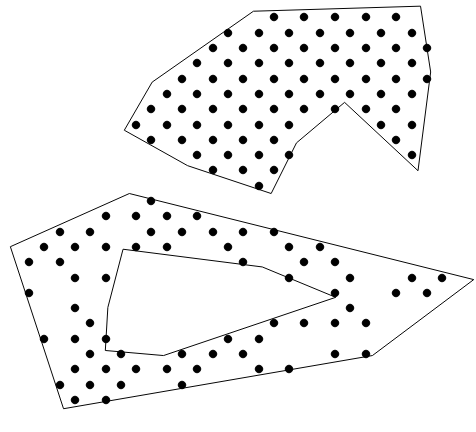
\includegraphics[width=.8\textwidth]{art/sampling.png}
\end{column}
\end{columns}

\begin{center}
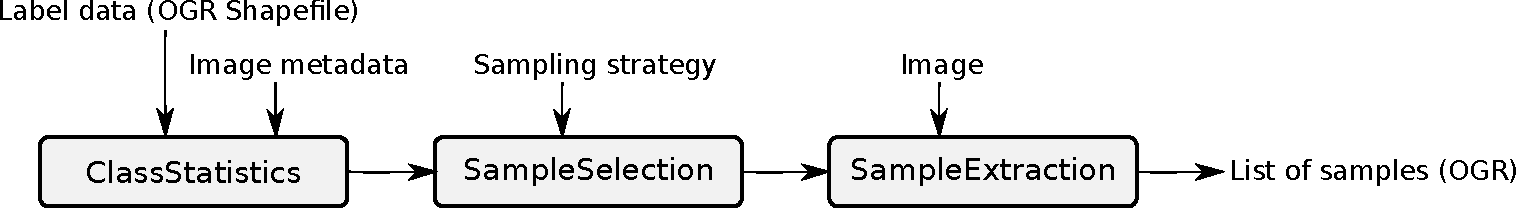
\includegraphics[width=\textwidth]{art/sampling_module.pdf}
\end{center}

\end{frame}

\begin{frame}
\frametitle{5.4 (Mai 2016)}
\begin{block}{OTB}
\begin{itemize}
\item Passage à un cycle de release fixe (3 mois)
\item Intégration du composant de visualisation
\item Compilation externe des modules externes
\item Nouvelles décompositions SAR: Barnes, Huynen, Pauli
\end{itemize}
\end{block}

\begin{block}{Monteverdi 3.2}
\begin{itemize}
\item Capture d'écran
\item Génération d'overviews GDAL
\item Gestion des sous datasets GDAL
\item Ajout au SuperBuild
\end{itemize}
\end{block}
\end{frame}

\section*{Conclusion}

\begin{frame}
\frametitle{Communauté OTB}
\begin{center}
Documentation, blog, wiki, git, bugtracker, dashboard, listes de diffusion:
{\huge\textcolor{red}{\href{http://www.orfeo-toolbox.org}{orfeo-toolbox.org}}}
\end{center}

\begin{block}{Évènements à venir:}
\begin{description}
\item[Journées Utilisateurs OTB] {Du 7 au 9 Juin 2016 à Toulouse}
\item[] {{\footnotesize\url{http://wiki.orfeo-toolbox.org/index.php/OTB\_Users\_meeting\_and\_hackfest\_2016}}}
\item[École d’été OTB et MicMac] {Du 4 au 8 Juillet 2016 à l'ENSG Paris}
\item[] {{\footnotesize\url{http://www.sfpt.fr/2016/04/ecole-dete-logiciels-libres-pour-le-traitement-des-images-satellites/}}}
\end{description}
\end{block}
\begin{center}

\includegraphics[scale=.3]{art/OSGeo_incubation.png}
\end{center}
\end{frame}

\end{document}
